\documentclass{ximera}  


%\usepackage{todonotes}
%\usepackage{mathtools} %% Required for wide table Curl and Greens
%\usepackage{cuted} %% Required for wide table Curl and Greens
\newcommand{\todo}{}

\usepackage{esint} % for \oiint
\ifxake%%https://math.meta.stackexchange.com/questions/9973/how-do-you-render-a-closed-surface-double-integral
\renewcommand{\oiint}{{\large\bigcirc}\kern-1.56em\iint}
\fi


\graphicspath{
  {./}
  {jpg}
  {ximeraTutorial/}
  {basicPhilosophy/}
  {functionsOfSeveralVariables/}
  {normalVectors/}
  {lagrangeMultipliers/}
  {vectorFields/}
  {greensTheorem/}
  {shapeOfThingsToCome/}
  {dotProducts/}
  {partialDerivativesAndTheGradientVector/}
  {../productAndQuotientRules/exercises/}
  {../motionAndPathsInSpace/exercises/}
  {../normalVectors/exercisesParametricPlots/}
  {../continuityOfFunctionsOfSeveralVariables/exercises/}
  {../partialDerivativesAndTheGradientVector/exercises/}
  {../directionalDerivativeAndChainRule/exercises/}
  {../commonCoordinates/exercisesCylindricalCoordinates/}
  {../commonCoordinates/exercisesSphericalCoordinates/}
  {../greensTheorem/exercisesCurlAndLineIntegrals/}
  {../greensTheorem/exercisesDivergenceAndLineIntegrals/}
  {../shapeOfThingsToCome/exercisesDivergenceTheorem/}
  {../greensTheorem/}
  {../shapeOfThingsToCome/}
  {../separableDifferentialEquations/exercises/}
  {vectorFields/}
}

\newcommand{\mooculus}{\textsf{\textbf{MOOC}\textnormal{\textsf{ULUS}}}}

\usepackage{tkz-euclide}\usepackage{tikz}
\usepackage{tikz-cd}
\usetikzlibrary{arrows}
\tikzset{>=stealth,commutative diagrams/.cd,
  arrow style=tikz,diagrams={>=stealth}} %% cool arrow head
\tikzset{shorten <>/.style={ shorten >=#1, shorten <=#1 } } %% allows shorter vectors

\usetikzlibrary{backgrounds} %% for boxes around graphs
\usetikzlibrary{shapes,positioning}  %% Clouds and stars
\usetikzlibrary{matrix} %% for matrix
\usepgfplotslibrary{polar} %% for polar plots
\usepgfplotslibrary{fillbetween} %% to shade area between curves in TikZ
\usetkzobj{all}
\usepackage[makeroom]{cancel} %% for strike outs
%\usepackage{mathtools} %% for pretty underbrace % Breaks Ximera
%\usepackage{multicol}
\usepackage{pgffor} %% required for integral for loops



%% http://tex.stackexchange.com/questions/66490/drawing-a-tikz-arc-specifying-the-center
%% Draws beach ball
\tikzset{pics/carc/.style args={#1:#2:#3}{code={\draw[pic actions] (#1:#3) arc(#1:#2:#3);}}}



\usepackage{array}
\setlength{\extrarowheight}{+.1cm}
\newdimen\digitwidth
\settowidth\digitwidth{9}
\def\divrule#1#2{
\noalign{\moveright#1\digitwidth
\vbox{\hrule width#2\digitwidth}}}





\newcommand{\RR}{\mathbb R}
\newcommand{\R}{\mathbb R}
\newcommand{\N}{\mathbb N}
\newcommand{\Z}{\mathbb Z}

\newcommand{\sagemath}{\textsf{SageMath}}


%\renewcommand{\d}{\,d\!}
\renewcommand{\d}{\mathop{}\!d}
\newcommand{\dd}[2][]{\frac{\d #1}{\d #2}}
\newcommand{\pp}[2][]{\frac{\partial #1}{\partial #2}}
\renewcommand{\l}{\ell}
\newcommand{\ddx}{\frac{d}{\d x}}

\newcommand{\zeroOverZero}{\ensuremath{\boldsymbol{\tfrac{0}{0}}}}
\newcommand{\inftyOverInfty}{\ensuremath{\boldsymbol{\tfrac{\infty}{\infty}}}}
\newcommand{\zeroOverInfty}{\ensuremath{\boldsymbol{\tfrac{0}{\infty}}}}
\newcommand{\zeroTimesInfty}{\ensuremath{\small\boldsymbol{0\cdot \infty}}}
\newcommand{\inftyMinusInfty}{\ensuremath{\small\boldsymbol{\infty - \infty}}}
\newcommand{\oneToInfty}{\ensuremath{\boldsymbol{1^\infty}}}
\newcommand{\zeroToZero}{\ensuremath{\boldsymbol{0^0}}}
\newcommand{\inftyToZero}{\ensuremath{\boldsymbol{\infty^0}}}



\newcommand{\numOverZero}{\ensuremath{\boldsymbol{\tfrac{\#}{0}}}}
\newcommand{\dfn}{\textbf}
%\newcommand{\unit}{\,\mathrm}
\newcommand{\unit}{\mathop{}\!\mathrm}
\newcommand{\eval}[1]{\bigg[ #1 \bigg]}
\newcommand{\seq}[1]{\left( #1 \right)}
\renewcommand{\epsilon}{\varepsilon}
\renewcommand{\phi}{\varphi}


\renewcommand{\iff}{\Leftrightarrow}

\DeclareMathOperator{\arccot}{arccot}
\DeclareMathOperator{\arcsec}{arcsec}
\DeclareMathOperator{\arccsc}{arccsc}
\DeclareMathOperator{\si}{Si}
\DeclareMathOperator{\scal}{scal}
\DeclareMathOperator{\sign}{sign}


%% \newcommand{\tightoverset}[2]{% for arrow vec
%%   \mathop{#2}\limits^{\vbox to -.5ex{\kern-0.75ex\hbox{$#1$}\vss}}}
\newcommand{\arrowvec}[1]{{\overset{\rightharpoonup}{#1}}}
%\renewcommand{\vec}[1]{\arrowvec{\mathbf{#1}}}
\renewcommand{\vec}[1]{{\overset{\boldsymbol{\rightharpoonup}}{\mathbf{#1}}}\hspace{0in}}

\newcommand{\point}[1]{\left(#1\right)} %this allows \vector{ to be changed to \vector{ with a quick find and replace
\newcommand{\pt}[1]{\mathbf{#1}} %this allows \vec{ to be changed to \vec{ with a quick find and replace
\newcommand{\Lim}[2]{\lim_{\point{#1} \to \point{#2}}} %Bart, I changed this to point since I want to use it.  It runs through both of the exercise and exerciseE files in limits section, which is why it was in each document to start with.

\DeclareMathOperator{\proj}{\mathbf{proj}}
\newcommand{\veci}{{\boldsymbol{\hat{\imath}}}}
\newcommand{\vecj}{{\boldsymbol{\hat{\jmath}}}}
\newcommand{\veck}{{\boldsymbol{\hat{k}}}}
\newcommand{\vecl}{\vec{\boldsymbol{\l}}}
\newcommand{\uvec}[1]{\mathbf{\hat{#1}}}
\newcommand{\utan}{\mathbf{\hat{t}}}
\newcommand{\unormal}{\mathbf{\hat{n}}}
\newcommand{\ubinormal}{\mathbf{\hat{b}}}

\newcommand{\dotp}{\bullet}
\newcommand{\cross}{\boldsymbol\times}
\newcommand{\grad}{\boldsymbol\nabla}
\newcommand{\divergence}{\grad\dotp}
\newcommand{\curl}{\grad\cross}
%\DeclareMathOperator{\divergence}{divergence}
%\DeclareMathOperator{\curl}[1]{\grad\cross #1}
\newcommand{\lto}{\mathop{\longrightarrow\,}\limits}

\renewcommand{\bar}{\overline}

\colorlet{textColor}{black}
\colorlet{background}{white}
\colorlet{penColor}{blue!50!black} % Color of a curve in a plot
\colorlet{penColor2}{red!50!black}% Color of a curve in a plot
\colorlet{penColor3}{red!50!blue} % Color of a curve in a plot
\colorlet{penColor4}{green!50!black} % Color of a curve in a plot
\colorlet{penColor5}{orange!80!black} % Color of a curve in a plot
\colorlet{penColor6}{yellow!70!black} % Color of a curve in a plot
\colorlet{fill1}{penColor!20} % Color of fill in a plot
\colorlet{fill2}{penColor2!20} % Color of fill in a plot
\colorlet{fillp}{fill1} % Color of positive area
\colorlet{filln}{penColor2!20} % Color of negative area
\colorlet{fill3}{penColor3!20} % Fill
\colorlet{fill4}{penColor4!20} % Fill
\colorlet{fill5}{penColor5!20} % Fill
\colorlet{gridColor}{gray!50} % Color of grid in a plot

\newcommand{\surfaceColor}{violet}
\newcommand{\surfaceColorTwo}{redyellow}
\newcommand{\sliceColor}{greenyellow}




\pgfmathdeclarefunction{gauss}{2}{% gives gaussian
  \pgfmathparse{1/(#2*sqrt(2*pi))*exp(-((x-#1)^2)/(2*#2^2))}%
}


%%%%%%%%%%%%%
%% Vectors
%%%%%%%%%%%%%

%% Simple horiz vectors
\renewcommand{\vector}[1]{\left\langle #1\right\rangle}


%% %% Complex Horiz Vectors with angle brackets
%% \makeatletter
%% \renewcommand{\vector}[2][ , ]{\left\langle%
%%   \def\nextitem{\def\nextitem{#1}}%
%%   \@for \el:=#2\do{\nextitem\el}\right\rangle%
%% }
%% \makeatother

%% %% Vertical Vectors
%% \def\vector#1{\begin{bmatrix}\vecListA#1,,\end{bmatrix}}
%% \def\vecListA#1,{\if,#1,\else #1\cr \expandafter \vecListA \fi}

%%%%%%%%%%%%%
%% End of vectors
%%%%%%%%%%%%%

%\newcommand{\fullwidth}{}
%\newcommand{\normalwidth}{}



%% makes a snazzy t-chart for evaluating functions
%\newenvironment{tchart}{\rowcolors{2}{}{background!90!textColor}\array}{\endarray}

%%This is to help with formatting on future title pages.
\newenvironment{sectionOutcomes}{}{}



%% Flowchart stuff
%\tikzstyle{startstop} = [rectangle, rounded corners, minimum width=3cm, minimum height=1cm,text centered, draw=black]
%\tikzstyle{question} = [rectangle, minimum width=3cm, minimum height=1cm, text centered, draw=black]
%\tikzstyle{decision} = [trapezium, trapezium left angle=70, trapezium right angle=110, minimum width=3cm, minimum height=1cm, text centered, draw=black]
%\tikzstyle{question} = [rectangle, rounded corners, minimum width=3cm, minimum height=1cm,text centered, draw=black]
%\tikzstyle{process} = [rectangle, minimum width=3cm, minimum height=1cm, text centered, draw=black]
%\tikzstyle{decision} = [trapezium, trapezium left angle=70, trapezium right angle=110, minimum width=3cm, minimum height=1cm, text centered, draw=black]




 
\title{Example Transmission Line Problem} 
\author{Milica Markovic} 
\outcome{Solve typical transmission-line problem.}
\begin{document}  
\begin{abstract}  

\end{abstract}  
\maketitle    


\begin{example}

A transmitter operated at 20MHz, Vg=100V with $Z_g=50 \Omega$ internal impedance is connected to an antenna load through l=6.33m of the line. The line is a lossless $Z_0=50 \Omega$, $\beta=0.595rad/m$. The antenna impedance at 20MHz measures $Z_L=36+j20 \Omega$. Set the beginning of the z-axis at the load, as shown in Figure \ref{fig:TRLine}.
\begin{enumerate}
\item What is the electrical length of the line? 
\item What is the input impedance of the line $Z_{in}$?
\item What is the forward going voltage at the load $\tilde{V}_0^+$?
\item Find the expression for forward voltage anywhere on the line.
\item Find the expression for reflected voltage anywhere on the line.
\item Find the total voltage anywhere on the line.
\item Find the expression for forward current anywhere on the line.
\item Find the expression for reflected current anywhere on the line.
\item Find the total current anywhere on the line.
\item Instead of the antenna, a load impedance $Z_l=50 \Omega$ is connected to this 50 Ohm line. How will that change the equations above?
\end{enumerate}




\begin{figure}[htbp]
\begin{center}
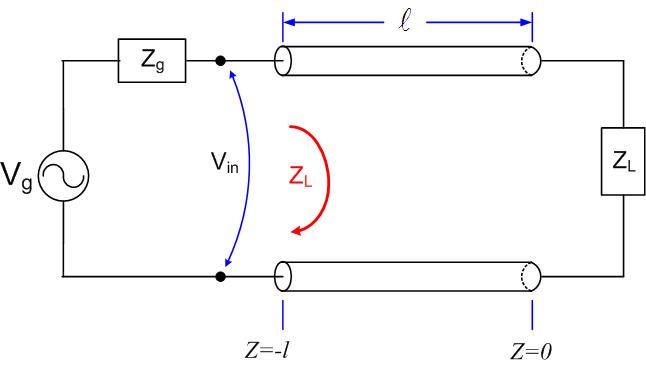
\includegraphics[scale=0.3]{../jpg/trline.jpg}
%\strut\psfig{figure=trline.ps,width=3cm} \\
\end{center}
\caption{Transmission Line connects generator and the load.}
\label{fig:TRLine}
\end{figure}


\begin{explanation}

The equations for the voltage and current anywhere (any z) on a transmission line  are


\begin{eqnarray}
\tilde{V}(z)= \tilde{V}_0^+ (e^{-j \beta z} + |\Gamma| e^{j(\beta z+\Theta_r)} ) \label{eq:vtlfin} \\
I(z)=   \frac{\tilde{V}_0^+}{Z_0}  (e^{-j \beta z} - \Gamma  e^{j \beta z}  ) \label{eq:itlfin}
\end{eqnarray}

We are given phase constant $\beta$, and we have to find the other unknowns: phasor of voltage at the load $\tilde{V}_0^+$, and the reflection coefficient $\Gamma$.    

Since we know the load impedance $Z_L$, and the transmission-line impedance $Z_0$, we can find the reflection coefficient $\Gamma$ using Equation \ref{eq:reflcoe1}.

\begin{eqnarray}
\Gamma=\frac{Z_L-Z_0}{Z_L+Z_0}
\approx-0.103130+j0.256542
\approx0.276495e^{j111.9001^\circ}
\approx0.276495e^{j1.953026} \label{eq:reflcoe1}
\end{eqnarray}

To find the input impedance of the line, we use the equation 


\begin{eqnarray}
Z_{in}= Z_0 \frac{Z_L+ j Z_0 \tan \beta l}{Z_0+ j Z_L \tan \beta l}
\approx(70.5267+j27.3178)\,\Omega
\end{eqnarray}

We can use one of the following two equations to find the forward going voltage at the load:

\begin{eqnarray}
\tilde{V}_0^+= \frac{\tilde{V}_g Z_{in}}{Z_g + Z_{in}} \frac{1}{e^{j \beta l} + \Gamma e^{-j \beta l}} \\
\tilde{V}_0^+=V_g e^{-j \beta l} \frac{Z_0}{Z_0 (1+\Gamma_{in}) +Z_g (1-\Gamma_{in})}
\end{eqnarray}

Because $Z_g=Z_0$, the denominator of the second expression is
$Z_0(1+\Gamma_{in})+Z_0(1-\Gamma_{in})=2Z_0$.
Thus $\tilde{V}_0^+=(V_g/2)e^{-j\beta l}$.
The specified values give $\beta l=0.595(6.33)=3.76635$ radians,
so $l/\lambda=\beta l/(2\pi)\approx0.599433$.
The forward voltage at the load is
$\tilde{V}_0^+=50e^{-j3.76635}\,\mathrm{V}$.



The equations of the voltage and current anywhere on the line are therefore

\begin{eqnarray}
\tilde{V}(z)\approx50e^{-j3.76635}
\left(e^{-j0.595z}+0.276495e^{j(0.595z+1.953026)}\right)\,\mathrm{V} \\
I(z)\approx e^{-j3.76635}
\left(e^{-j0.595z}-0.276495e^{j(0.595z+1.953026)}\right)\,\mathrm{A}
\end{eqnarray}

Suppose we replace the antenna with another load of impedance
$50\Omega$. The load reflection coefficient is then zero, and
both reflected waves vanish. The total voltage equals the
forward voltage, and the total current equals the forward
current, which is the forward voltage divided by $Z_0$.


\begin{eqnarray}
\tilde{V}(z)= \tilde{V}_0^+ e^{-j \beta z}   \\
I(z)=   \frac{\tilde{V}_0^+}{Z_0}  e^{-j \beta z} 
\end{eqnarray}


\end{explanation}




\end{example}






\end{document} 
